%===================================================================================
\chapter{Mathematical Considerations}\label{s:math}
%===================================================================================

{\idas} solves the initial-value problem (IVP) for a DAE system of the
general form
\begin{equation}\label{e:DAE}
  F(t,y,\dot{y}) = 0 \, ,
  \quad y(t_0) = y_0 \, ,~ \dot{y}(t_0) = \dot{y}_0 \, ,
\end{equation}
where $y$, $\dot{y}$, and $F$ are vectors in ${\bf R}^N$, $t$ is the independent
variable, $\dot{y} = dy/dt$, and initial values $y_0$, $\dot{y}_0$ 
are given.  (Often $t$ is time, but it certainly need not be.)

Additionally, if (\ref{e:DAE}) depends on some parameters $p \in {\bf R}^{N_p}$,
i.e.
\begin{equation}\label{e:DAE_p}
\begin{split}
& F(t, y, \dot y , p) = 0 \\
& y(t_0) = y_0(p) \, ,~ {\dot y}(t_0) = \dot y_0(p) \, ,
\end{split}
\end{equation}
{\idas} can also compute first order derivative information, performing either
{\em forward sensitivity analysis} or {\em adjoint sensitivity analysis}.
In the first case, {\idas} computes the sensitivities of the
solution with respect to the parameters $p$, while in the second case,
{\idas} computes the gradient of a {\em derived function} with
respect to the parameters $p$.


%------------------------
\section{IVP solution}\label{ss:ivp_sol}
%------------------------

% Initial condition calculation
%------------------------------
Prior to integrating a DAE initial-value problem, an important requirement 
is that the pair of vectors $y_0$ and $\dot{y}_0$ are both initialized to
satisfy the DAE residual $F(t_0,y_0, \dot{y}_0) = 0$.
For a class of problems that includes so-called
semi-explicit index-one systems, {\idas} provides a routine that computes
consistent initial conditions from a user's initial guess~\cite{BHP:98}.  
For this, the user must identify sub-vectors of $y$
(not necessarily contiguous), denoted $y_d$ and $y_a$, which are its
differential and algebraic parts, respectively, such that $F$ depends
on $\dot{y}_d$ but not on any components of $\dot{y}_a$.  The assumption that
the system is ``index one'' means that for a given $t$ and $y_d$, the
system $F(t,y,\dot{y}) = 0$ defines $y_a$ uniquely.  In this case, a solver
within {\idas} computes $y_a$ and $\dot{y}_d$ at $t = t_0$, given $y_d$ and an
initial guess for $y_a$.  A second available option with this solver
also computes all of $y(t_0)$ given $\dot{y}(t_0)$; this is intended mainly
for quasi-steady-state problems, where $\dot{y}(t_0) = 0$ is given.
In both cases, {\ida} solves the system $F(t_0,y_0, \dot{y}_0) = 0$ for the
unknown components of $y_0$ and $\dot{y}_0$, using Newton iteration
augmented with a line search global strategy.  In doing this, it makes
use of the existing machinery that is to be used for solving the
linear systems during the integration, in combination with certain
tricks involving the step size (which is set artificially for this
calculation).
For problems that do not fall into either of these categories, the
user is responsible for passing consistent values, or risks failure in
the numerical integration.

% Integration method and nonlinear system
%----------------------------------------
The integration method used in {\idas} is the variable-order, variable-coefficient
BDF (Backward Differentiation Formula), in fixed-leading-coefficient
form~\cite{BCP:96}.
The method order ranges from 1 to 5, with the BDF of order $q$
given by the multistep formula
\begin{equation}\label{e:BDF}
  \sum_{i=0}^q \alpha_{n,i}y_{n-i} = h_n \dot{y}_n \, ,
\end{equation}
where $y_n$ and $\dot{y}_n$ are the computed approximations to $y(t_n)$
and $\dot{y}(t_n)$, respectively, and the step size is $h_n = t_n - t_{n-1}$.  
The coefficients $\alpha_{n,i}$ are uniquely determined by the order
$q$, and the history of the step sizes.  The application of the BDF
(\ref{e:BDF}) to the DAE system (\ref{e:DAE}) results in a nonlinear
algebraic system to be solved at each step:
\begin{equation}\label{e:DAE_nls}
  G(y_n) \equiv 
  F \left( t_n , \, y_n , \, 
    h_n^{-1} \sum_{i=0}^q \alpha_{n,i}y_{n-i} \right) = 0 \, .
\end{equation}
%
Regardless of the method options, the solution of the nonlinear system
(\ref{e:DAE_nls}) is accomplished with some form of Newton iteration.
This leads to a linear system for each Newton correction, of the form
\begin{equation}\label{e:DAE_Newtoncorr}
  J [y_{n(m+1)} - y_{n(m)}] = -G(y_{n(m)})  \, , 
\end{equation}
where $y_{n(m)}$ is the $m$-th approximation to $y_n$. 
%
Here $J$ is some approximation to the system Jacobian
\begin{equation}\label{e:DAE_Jacobian}
  J = \frac{\partial G}{\partial y}
  = \frac{\partial F}{\partial y} + 
  \alpha\frac{\partial F}{\partial \dot{y}} \, ,
\end{equation}
where $\alpha = \alpha_{n,0}/h_n$.  The scalar $\alpha$ changes 
whenever the step size or method order changes.

For the solution of the linear systems within the Newton corrections, 
{\idas} provides several choices, including the option of an user-supplied
linear solver module. The linear solver modules distributed with {\sundials}
are organized in two families, a {\em direct} family comprising direct linear 
solvers for dense, banded, or sparse matrices and a {\em spils} family comprising
scaled preconditioned iterative (Krylov) linear solvers. 
%%
The methods offered through these modules are as follows:
\begin{itemize}
\item dense direct solvers, using either an internal implementation or 
  a Blas/Lapack implementation (serial or threaded vector modules only),
\item band direct solvers, using either an internal implementation or 
  a Blas/Lapack implementation (serial or threaded vector modules only),
\item sparse direct solver interfaces, using either the KLU sparse solver
  library \cite{DaPa:10,KLU_site}, or the thread-enabled SuperLU\_MT sparse
  solver library \cite{Li:05,DGL:99,SuperLUMT_site} (serial or threaded 
  vector modules only) [Note that users will need to download and install the 
  {\klu} or {\superlumt} packages independent of {\idas}],
\item {\spgmr}, a scaled preconditioned GMRES (Generalized Minimal Residual method)
  solver without restarts,
\item {\spfgmr}, a scaled preconditioned FGMRES (Flexible Generalized
  Minimal Residual method) solver,
\item {\spbcg}, a scaled preconditioned Bi-CGStab (Bi-Conjugate Gradient Stable
  method) solver,
\item {\sptfqmr}, a scaled preconditioned TFQMR (Transpose-Free Quasi-Minimal
  Residual method) solver, or
\item {\pcg}, a scaled preconditioned CG (Conjugate Gradient method) solver.
\end{itemize}
For large stiff systems, where direct methods are not feasible, the
combination of a BDF integrator and any of the preconditioned Krylov
methods ({\spgmr}, {\spbcg}, or {\sptfqmr}) yields a powerful tool
because it combines established methods for stiff integration,
nonlinear iteration, and Krylov (linear) iteration with a
problem-specific treatment of the dominant source of stiffness, in the
form of the user-supplied preconditioner matrix \cite{BrHi:89}. 
For the {\em spils} linear solvers,  preconditioning is allowed
only on the left (see \S\ref{s:preconditioning}).
%%
Note that the dense, band, and sparse direct linear solvers can only be 
used with serial and threaded vector representations.

% WRMS Norm
%----------
\index{weighted root-mean-square norm|(}
In the process of controlling errors at various levels, {\idas} uses a
weighted root-mean-square norm, denoted $\|\cdot\|_{\mbox{\scriptsize WRMS}}$,
for all error-like quantities.  The multiplicative weights used are based on
the current solution and on the relative and absolute tolerances input by the
user, namely
\index{tolerances}
\begin{equation}\label{e:errwt}
 W_i = 1 / [ \mbox{\sc rtol} \cdot |y_i| + \mbox{\sc atol}_i ] \, .
\end{equation}
Because $1/W_i$ represents a tolerance in the component $y_i$, a vector
whose norm is 1 is regarded as ``small.''  For brevity, we will
usually drop the subscript WRMS on norms in what follows.
\index{weighted root-mean-square norm|)}

% Newton iteration
%-----------------
In the case of a direct linear solver (dense, band, or sparse), the nonlinear 
iteration (\ref{e:DAE_Newtoncorr}) is a Modified Newton iteration, in
that the Jacobian $J$ is fixed (and usually out of date), with a coefficient 
$\bar\alpha$ in place of $\alpha$ in $J$. When using one of the Krylov methods
{\spgmr}, {\spbcg}, or {\sptfqmr} as the linear solver, the iteration is an
Inexact Newton iteration, using the current Jacobian (through matrix-free products
$Jv$), in which the linear residual $J\Delta y + G$ is nonzero but controlled.
The Jacobian matrix $J$ (direct cases) or preconditioner matrix $P$ 
({\spgmr}/{\spbcg}/{\sptfqmr} case) is updated when:
\begin{itemize}
\item starting the problem,
\item the value $\bar\alpha$ at the last update is such that
  $\alpha / {\bar\alpha} < 3/5$ or $\alpha / {\bar\alpha} > 5/3$, or
\item a non-fatal convergence failure occurred with an out-of-date $J$ or $P$.
\end{itemize}
The above strategy balances the high cost of frequent matrix evaluations
and preprocessing with the slow convergence due to infrequent updates.
To reduce storage costs on an update, Jacobian information is always
reevaluated from scratch.

We note that with the sparse direct solvers, the Jacobian {\em must}
be supplied by a user routine in compressed-sparse-column format, as
this is not approximated automatically within {\idas}.


% Newton convergence test
%------------------------
The stopping test for the Newton iteration
in {\idas} ensures that the iteration error $y_n - y_{n(m)}$ is small relative
to $y$ itself. For this, we estimate the linear convergence rate at all 
iterations $m>1$ as
\begin{equation*}
R = \left( \frac{\delta_m}{\delta_1} \right)^{\frac{1}{m-1}} \, , 
\end{equation*}
where the $\delta_m = y_{n(m)} - y_{n(m-1)}$ is the correction at
iteration $m=1,2,\ldots$. The Newton iteration is halted if $R>0.9$.
The convergence test at the $m$-th iteration is then
\begin{equation}\label{e:DAE_nls_test}
S \| \delta_m \| < 0.33 \, ,
\end{equation}
where $S = R/(R-1)$ whenever $m>1$ and $R\le 0.9$. The user has the
option of changing the constant in the convergence test from its default 
value of $0.33$.
%
The quantity $S$ is set to $S=20$ initially and whenever $J$ or $P$ is
updated, and it is reset to $S=100$ on a step with $\alpha \neq \bar\alpha$.
Note that at $m=1$, the convergence test (\ref{e:DAE_nls_test}) uses an old 
value for $S$. Therefore, at the first Newton iteration, we make an additional
test and stop the iteration if $\|\delta_1\| < 0.33 \cdot 10^{-4}$
(since such a $\delta_1$ is probably just noise and therefore not appropriate 
for use in evaluating $R$).
%
We allow only a small number (default value 4) of Newton iterations.
If convergence fails with $J$ or $P$ current, 
we are forced to reduce the step size $h_n$, and we replace $h_n$ by $h_n/4$.
The integration is halted after a preset number (default value 10)
of convergence failures. Both the maximum allowable Newton iterations
and the maximum nonlinear convergence failures can be changed by the user
from their default values.

When {\spgmr}, {\spbcg}, or {\sptfqmr} is used to solve the linear system, to
minimize the effect of linear iteration errors on the nonlinear and local integration
error controls, we require the preconditioned linear residual to be small relative to
the allowed error in the Newton iteration, i.e., 
$\| P^{-1}(Jx+G) \| < 0.05 \cdot 0.33$.
The safety factor $0.05$ can be changed by the user.

% Jacobian DQ approximations
%---------------------------
In the direct linear solver 
cases, the Jacobian $J$ defined in (\ref{e:DAE_Jacobian}) 
can be either supplied by the user or have {\idas} compute one internally 
by difference quotients. In the latter case, we use the approximation
\begin{gather*}
  J_{ij} = [F_i(t,y+\sigma_j e_j,\dot{y}+\alpha\sigma_j e_j) - 
            F_i(t,y,\dot{y})]/\sigma_j \, , \text{ with}\\
  \sigma_j = \sqrt{U} \max \left\{ |y_j|, |h\dot{y}_j|,1/W_j \right\}
             \mbox{sign}(h \dot{y}_j) \, ,
\end{gather*}
where $U$ is the unit roundoff, $h$ is the current step size, and $W_j$ is 
the error weight for the component $y_j$ defined by (\ref{e:errwt}).
In the {\spgmr}/{\spbcg}/{\sptfqmr} case, if a routine for $Jv$ is not
supplied, such products are approximated by
\begin{equation*}
Jv = [F(t,y+\sigma v,\dot{y}+\alpha\sigma v) - F(t,y,\dot{y})]/\sigma \, ,
\end{equation*}
where the increment $\sigma$ is $1/\|v\|$.  As an option, the user can
specify a constant factor that is inserted into this expression for $\sigma$.

% Error control
%--------------
During the course of integrating the system, {\idas} computes an estimate
of the local truncation error, LTE, at the $n$-th time step, and
requires this to satisfy the inequality
\begin{equation*}
  \| \mbox{LTE} \|_{\mbox{\scriptsize WRMS}} \leq 1 \, .               
\end{equation*}
Asymptotically, LTE varies as $h^{q+1}$ at step size $h$ and order $q$, as
does the predictor-corrector difference $\Delta_n \equiv y_n-y_{n(0)}$.  
Thus there is a constant $C$ such that
\[ \mbox{LTE} = C \Delta_n + O(h^{q+2}) \, , \]
and so the norm of LTE is estimated as $|C| \cdot \|\Delta_n\|$.
In addition, {\idas} requires that the error in the associated polynomial
interpolant over the current step be bounded by 1 in norm.  The
leading term of the norm of this error is bounded by
$\bar{C} \|\Delta_n\|$ for another constant $\bar{C}$.  Thus the local
error test in {\idas} is
\begin{equation}\label{lerrtest}
   \max\{ |C|, \bar{C} \} \|\Delta_n\| \leq 1 \, .
\end{equation}
A user option is available by which the algebraic components of the
error vector are omitted from the test (\ref{lerrtest}), if these have
been so identified.

% Step/order selection
%---------------------
In {\idas}, the local error test is tightly coupled with the logic for
selecting the step size and order.  First, there is an initial phase
that is treated specially; for the first few steps, the step size is
doubled and the order raised (from its initial value of 1) on every
step, until (a) the local error test (\ref{lerrtest}) fails, (b) the
order is reduced (by the rules given below), or (c) the order reaches
5 (the maximum).  For step and order selection on the general step,
{\idas} uses a different set of local error estimates, based on the
asymptotic behavior of the local error in the case of fixed step sizes.
At each of the orders $q'$ equal to $q$, $q-1$ (if $q > 1$), $q-2$ (if
$q > 2$), or $q+1$ (if $q < 5$), there are constants $C(q')$ such that
the norm of the local truncation error at order $q'$ satisfies
\[ \mbox{LTE}(q') = C(q') \| \phi(q'+1) \| + O(h^{q'+2}) \, , \]
where $\phi(k)$ is a modified divided difference of order $k$ that is
retained by {\idas} (and behaves asymptotically as $h^k$).
Thus the local truncation errors are estimated as
ELTE$(q') = C(q')\|\phi(q'+1)\|$ to select step sizes.  But the choice
of order in {\idas} is based on the requirement that the scaled derivative
norms, $\|h^k y^{(k)}\|$, are monotonically decreasing with $k$, for
$k$ near $q$.  These norms are again estimated using the $\phi(k)$,
and in fact
\[ \|h^{q'+1} y^{(q'+1)}\| \approx T(q') \equiv (q'+1) \mbox{ELTE}(q') \, . \]
The step/order selection begins with a test for monotonicity that is
made even {\em before} the local error test is performed.  Namely,
the order is reset to $q' = q-1$ if (a) $q=2$ and $T(1)\leq T(2)/2$,
or (b) $q > 2$ and $\max\{T(q-1),T(q-2)\} \leq T(q)$; otherwise 
$q' = q$.  Next the local error test (\ref{lerrtest}) is performed,
and if it fails, the step is redone at order $q\leftarrow q'$ and a
new step size $h'$.  The latter is based on the $h^{q+1}$ asymptotic
behavior of $\mbox{ELTE}(q)$, and, with safety factors, is given by
\[ \eta = h'/h = 0.9/[2 \, \mbox{ELTE}(q)]^{1/(q+1)} \, . \]
The value of $\eta$ is adjusted so that $0.25 \leq \eta \leq 0.9$
before setting $h \leftarrow h' = \eta h$.  If the local error test
fails a second time, {\idas} uses $\eta = 0.25$, and on the third
and subsequent failures it uses $q = 1$ and $\eta = 0.25$.  After
10 failures, {\idas} returns with a give-up message.

As soon as the local error test has passed, the step and order for the
next step may be adjusted.  No such change is made if $q' = q-1$ from
the prior test, if $q = 5$, or if $q$ was increased on the previous
step.  Otherwise, if the last $q+1$ steps were taken at a constant
order $q < 5$ and a constant step size, {\idas} considers raising the order
to $q+1$.  The logic is as follows: (a) If $q = 1$, then reset $q = 2$
if $T(2) < T(1)/2$.  (b) If $q > 1$ then 
\begin{itemize}
\item reset $q \leftarrow q-1$ if $T(q-1) \leq \min\{T(q),T(q+1)\}$;
\item else reset $q \leftarrow q+1$ if $T(q+1) < T(q)$;
\item leave $q$ unchanged otherwise $[$then $T(q-1) > T(q) \leq T(q+1)]$.
\end{itemize}
In any case, the new step size $h'$ is set much as before:
\[ \eta = h'/h = 1/[2 \, \mbox{ELTE}(q)]^{1/(q+1)} \, . \]
The value of $\eta$ is adjusted such that (a) if $\eta > 2$, $\eta$ is
reset to 2; (b) if $\eta \leq 1$, $\eta$ is restricted to 
$0.5 \leq \eta \leq 0.9$; and (c) if $1 < \eta < 2$ we use $\eta = 1$.
Finally $h$ is reset to $h' = \eta h$.  Thus we do not increase the
step size unless it can be doubled.  See \cite{BCP:96} for details.

% Additional constraints on y components
%---------------------------------------
{\idas} permits the user to impose optional inequality constraints on individual 
components of the solution vector $y$. Any of the following four constraints 
can be imposed: $y_i > 0$, $y_i < 0$, $y_i \geq 0$, or $y_i \leq 0$. 
The constraint satisfaction is tested after a successful nonlinear system solution. 
If any constraint fails, we declare a convergence failure of the Newton iteration 
and reduce the step size. Rather than cutting the step size by some arbitrary factor, 
{\idas} estimates a new step size $h'$ using a linear approximation of the components 
in $y$ that failed the constraint test (including a safety factor of $0.9$ to 
cover the strict inequality case). These additional constraints are also imposed
during the calculation of consistent initial conditions.

Normally, {\idas} takes steps until a user-defined output value $t =
t_{\mbox{\scriptsize out}}$ is overtaken, and then computes
$y(t_{\mbox{\scriptsize out}})$ by interpolation.  However, a
``one step'' mode option is available, where control returns to the
calling program after each step.  There are also options to force {\idas}
not to integrate past a given stopping point $t = t_{\mbox{\scriptsize
stop}}$.


%------------------------
\section{Preconditioning}\label{s:preconditioning}
%------------------------
\index{preconditioning!advice on|(}
When using a Newton method to solve the nonlinear system (\ref{e:DAE_Newtoncorr}),
{\idas} makes repeated use of a linear solver to solve linear systems of the form
$J \Delta y = - G$.
If this linear system solve is done with one of the scaled preconditioned iterative 
linear solvers, these solvers are rarely successful if used without preconditioning;
it is generally necessary to precondition the system in order to obtain acceptable efficiency.  
A system $A x = b$ can be preconditioned on the left, on the right,
or on both sides. The Krylov method is then applied to a system with the matrix $P^{-1}A$, 
or $AP^{-1}$, or $P_L^{-1} A P_R^{-1}$, instead of $A$.  
However, within {\idas}, preconditioning is allowed {\em only} on the left,
so that the iterative method is applied to systems $(P^{-1}J)\Delta y = -P^{-1}G$.  
Left preconditioning is required to make the norm of the linear residual in the Newton 
iteration meaningful; in general, $\| J \Delta y + G \|$ is meaningless, since the 
weights used in the WRMS-norm correspond to $y$.

In order to improve the convergence of the Krylov iteration, the preconditioner matrix 
$P$ should in some sense approximate the system matrix $A$.  
Yet at the same time, in order to be cost-effective, the matrix $P$ should
be reasonably efficient to evaluate and solve.  Finding a good point
in this tradeoff between rapid convergence and low cost can be very
difficult.  Good choices are often problem-dependent (for example, see
\cite{BrHi:89} for an extensive study of preconditioners for
reaction-transport systems).

Typical preconditioners used with {\idas} are based on approximations to the Newton 
iteration matrix of the systems involved; in other words, 
$P \approx \frac{\partial F}{\partial y} + \alpha\frac{\partial F}{\partial \dot{y}}$,
where $\alpha$ is a scalar inversely proportional to the integration step size $h$.
Because the Krylov iteration occurs within a Newton iteration and further
also within a time integration, and since each of these iterations has
its own test for convergence, the preconditioner may use a very crude
approximation, as long as it captures the dominant numerical
feature(s) of the system.  We have found that the combination of a
preconditioner with the Newton-Krylov iteration, using even a fairly
poor approximation to the Jacobian, can be surprisingly superior to
using the same matrix without Krylov acceleration (i.e., a modified
Newton iteration), as well as to using the Newton-Krylov method with
no preconditioning.
\index{preconditioning!advice on|)}

%------------------------
\section{Rootfinding}\label{s:rootfinding}
%------------------------

\index{Rootfinding}
The {\idas} solver has been augmented to include a rootfinding
feature.  This means that, while integrating the Initial Value Problem
(\ref{e:DAE}), {\idas} can also find the roots of a set of user-defined
functions $g_i(t,y,\dot{y})$ that depend on $t$, the solution vector 
$y = y(t)$, and its $t-$derivative $\dot{y}(t)$.  The number of these root
functions is arbitrary, and if more than one $g_i$ is found to have a
root in any given interval, the various root locations are found and
reported in the order that they occur on the $t$ axis, in the
direction of integration.

Generally, this rootfinding feature finds only roots of odd
multiplicity, corresponding to changes in sign of $g_i(t,y(t),\dot{y}(t))$,
denoted $g_i(t)$ for short.  If a user root function has a root of
even multiplicity (no sign change), it will probably be missed by
{\idas}.  If such a root is desired, the user should reformulate the
root function so that it changes sign at the desired root.

The basic scheme used is to check for sign changes of any $g_i(t)$ over
each time step taken, and then (when a sign change is found) to home
in on the root (or roots) with a modified secant method \cite{HeSh:80}.  
In addition, each time $g$ is computed, {\idas} checks to see if 
$g_i(t) = 0$ exactly, and if so it reports this as a root.  However,
if an exact zero of any $g_i$ is found at a point $t$, {\idas}
computes $g$ at $t + \delta$ for a small increment $\delta$, slightly
further in the direction of integration, and if any $g_i(t + \delta)=0$ 
also, {\idas} stops and reports an error.  This way, each time
{\idas} takes a time step, it is guaranteed that the values of all
$g_i$ are nonzero at some past value of $t$, beyond which a search for
roots is to be done.

At any given time in the course of the time-stepping, after suitable
checking and adjusting has been done, {\idas} has an interval
$(t_{lo},t_{hi}]$ in which roots of the $g_i(t)$ are to be sought, such
that $t_{hi}$ is further ahead in the direction of integration, and
all $g_i(t_{lo}) \neq 0$.  The endpoint $t_{hi}$ is either $t_n$,
the end of the time step last taken, or the next requested output time
$t_{\mbox{\scriptsize out}}$ if this comes sooner.  The endpoint
$t_{lo}$ is either $t_{n-1}$, or the last output time
$t_{\mbox{\scriptsize out}}$ (if this occurred within the last
step), or the last root location (if a root was just located within
this step), possibly adjusted slightly toward $t_n$ if an exact zero
was found.  The algorithm checks $g$ at $t_{hi}$ for zeros and for
sign changes in $(t_{lo},t_{hi})$.  If no sign changes are found, then
either a root is reported (if some $g_i(t_{hi}) = 0$) or we proceed to
the next time interval (starting at $t_{hi}$).  If one or more sign
changes were found, then a loop is entered to locate the root to
within a rather tight tolerance, given by
\[ \tau = 100 * U * (|t_n| + |h|)~~~ (U = \mbox{unit roundoff}) ~. \]
Whenever sign changes are seen in two or more root functions, the one
deemed most likely to have its root occur first is the one with the
largest value of $|g_i(t_{hi})|/|g_i(t_{hi}) - g_i(t_{lo})|$,
corresponding to the closest to $t_{lo}$ of the secant method values.
At each pass through the loop, a new value $t_{mid}$ is set, strictly
within the search interval, and the values of $g_i(t_{mid})$ are
checked.  Then either $t_{lo}$ or $t_{hi}$ is reset to $t_{mid}$
according to which subinterval is found to have the sign change.  If
there is none in $(t_{lo},t_{mid})$ but some $g_i(t_{mid}) = 0$, then
that root is reported.  The loop continues until 
$|t_{hi}-t_{lo}| < \tau$, and then the reported root location is
$t_{hi}$.

In the loop to locate the root of $g_i(t)$, the formula for $t_{mid}$
is
\[ t_{mid} = t_{hi} - (t_{hi} - t_{lo})
             g_i(t_{hi}) / [g_i(t_{hi}) - \alpha g_i(t_{lo})] ~, \] 
where $\alpha$ a weight parameter.  On the first two passes through
the loop, $\alpha$ is set to $1$, making $t_{mid}$ the secant method
value.  Thereafter, $\alpha$ is reset according to the side of the
subinterval (low vs high, i.e. toward $t_{lo}$ vs toward $t_{hi}$)
in which the sign change was found in the previous two passes.  If the
two sides were opposite, $\alpha$ is set to 1.  If the two sides were
the same, $\alpha$ is halved (if on the low side) or doubled (if on
the high side).  The value of $t_{mid}$ is closer to $t_{lo}$ when
$\alpha < 1$ and closer to $t_{hi}$ when $\alpha > 1$.  If the above
value of $t_{mid}$ is within $\tau/2$ of $t_{lo}$ or $t_{hi}$, it is
adjusted inward, such that its fractional distance from the endpoint
(relative to the interval size) is between .1 and .5 (.5 being the
midpoint), and the actual distance from the endpoint is at least
$\tau/2$.

%----------------------------------------
\section{Pure quadrature integration}\label{s:quad}
%----------------------------------------

\index{quadrature integration}
In many applications, and most notably during the backward integration phase
of an adjoint sensitivity analysis run (see \S\ref{ss:adj_sensi}) it is of
interest to compute integral quantities of the form
\begin{equation}\label{e:QUAD}
  z(t) = \int_{t_0}^t q(\tau, y(\tau), \dot{y}(\tau), p) \, d\tau \, .
\end{equation}
The most effective approach to compute $z(t)$ is to extend the original problem
with the additional ODEs (obtained by applying Leibnitz's differentiation rule):
\begin{equation}
  \dot z = q(t,y,\dot{y},p) \, , \quad z(t_0) = 0 \, .
\end{equation}
Note that this is equivalent to using a quadrature method based on the underlying
linear multistep polynomial representation for $y(t)$.

This can be done at the ``user level'' by simply exposing to {\idas} the extended 
DAE system (\ref{e:DAE_p})+(\ref{e:QUAD}). However, in the context of an implicit 
integration solver, this approach is not desirable since the nonlinear solver 
module will require the Jacobian (or Jacobian-vector product) of this extended DAE.
Moreover, since the additional states, $z$, do not enter the right-hand side of
the ODE (\ref{e:QUAD}) and therefore the residual of the extended DAE system
does not depend on $z$, it is much more efficient to treat the ODE system (\ref{e:QUAD})
separately from the original DAE system (\ref{e:DAE_p}) by ``taking out'' the additional
states $z$ from the nonlinear system (\ref{e:DAE_nls}) that must be solved in
the correction step of the LMM. Instead, ``corrected'' values $z_n$ are computed
explicitly as
\begin{equation*}
  z_n = \frac{1}{\alpha_{n,0}} \left(
    h_n q(t_n, y_n, \dot{y}_n, p) - \sum_{i=1}^q \alpha_{n,i} z_{n-i}
    \right) \, ,
\end{equation*}
once the new approximation $y_n$ is available.

The quadrature variables $z$ can be optionally included in the error test, in 
which case corresponding relative and absolute tolerances must be provided.


%----------------------------------------
\section{Forward sensitivity analysis}\label{ss:fwd_sensi}
%----------------------------------------

\index{forward sensitivity analysis!mathematical background|(}
Typically, the governing equations of complex, large-scale models
depend on various parameters,  through the right-hand side vector 
and/or through the vector of initial conditions, as in (\ref{e:DAE_p}).
In addition to numerically solving the DAEs, it may be desirable to
determine the sensitivity of the results with respect to the model
parameters. 
Such sensitivity information can be used to estimate which
parameters are most influential in affecting the behavior of the
simulation or to evaluate optimization gradients (in the setting of dynamic
optimization, parameter estimation, optimal control, etc.).

The {\em solution sensitivity} with respect to the model parameter
$p_i$ is defined as the vector 
$s_i (t) = {\partial y(t)}/{\partial p_i}$
and satisfies the following {\em forward sensitivity equations}
(or {\em sensitivity equations} for short):
\begin{equation}\label{e:sens_eqns}
\begin{split}
& \frac{\partial F}{\partial y} s_i + \frac{\partial F}{\partial \dot y} {\dot s_i} + \frac{\partial F}{\partial p_i} = 0\\
& s_i(t_0) = \frac{\partial y_{0}(p)}{\partial p_i} \, ,~ \dot s_i(t_0) =  \frac{\partial \dot y_{0}(p)}{\partial p_i} \, ,
\end{split}
\end{equation}
obtained by applying the chain rule of differentiation to the original DAEs~(\ref{e:DAE_p}). 


When performing forward sensitivity analysis, {\idas} carries out
the time integration of the combined system, (\ref{e:DAE_p}) and
(\ref{e:sens_eqns}), by viewing it as a DAE system of size
$N(N_s+1)$, where $N_s$ is the number of model parameters $p_i$, with
respect to which sensitivities are desired ($N_s \le N_p$).
However, major improvements in efficiency can be made by taking
advantage of the special form of the sensitivity equations as
linearizations of the original DAEs.  In particular, the original
DAE system and all sensitivity systems share the same Jacobian matrix
$J$ in (\ref{e:DAE_Jacobian}).

The sensitivity equations are solved with the same linear multistep formula that
was selected for the original DAEs and the same linear solver is used in the correction
phase for both state and sensitivity variables. In addition, {\idas} offers the option of
including ({\em full error control}) or excluding ({\em partial error control}) the
sensitivity variables from the local error test.

\subsection{Forward sensitivity methods}
\index{forward sensitivity analysis!correction strategies|(}
In what follows we briefly describe three methods that have been proposed for the 
solution of the combined DAE and sensitivity system for the vector
${\hat y} = [y, s_1, \ldots , s_{N_s}]$.

\begin{itemize}

\item {\em Staggered Direct}
  %%
  In this approach \cite{CaSt:85}, the nonlinear system (\ref{e:DAE_nls}) is first
  solved and, once an acceptable numerical solution is obtained, the sensitivity 
  variables at the new step are found by directly solving (\ref{e:sens_eqns}) 
  after the BDF discretization is used to eliminate ${\dot s}_i$. 
  Although the system matrix of the above linear system is based on exactly the same
  information as the matrix $J$ in (\ref{e:DAE_Jacobian}), it must be updated and
  factored at every step of the integration, in contrast to an evaluation of
  $J$ which is updated only occasionally.  For problems with many parameters
  (relative to the problem size), the staggered direct method can outperform
  the methods described  below~\cite{LPZ:99}.
  However, the computational cost associated with matrix updates and factorizations 
  makes this method unattractive for problems with many more states than parameters
  (such as those arising from semidiscretization of PDEs) and is therefore not 
  implemented in {\idas}.
  
\item {\em Simultaneous Corrector}
  %%
  In this method \cite{MaPe:97}, the discretization is applied simultaneously
  to both the original equations (\ref{e:DAE_p}) and the sensitivity systems
  (\ref{e:sens_eqns}) resulting in an ``extended'' nonlinear system ${\hat G}({\hat y}_n) = 0$
  where ${\hat y_n} = [ y_n, \ldots, s_i, \ldots ]$.
  This combined nonlinear system can be solved using a modified Newton method as in
  (\ref{e:DAE_Newtoncorr}) by solving the corrector equation
  \begin{equation}\label{e:Newton_sim}
    {\hat J}[{\hat y}_{n(m+1)}-{\hat y}_{n(m)}]=-{\hat G}({\hat y}_{n(m)})
  \end{equation}
  at each iteration, where 
  \begin{equation*}
    {\hat J} = 
    \begin{bmatrix}
      J       &        &        &        &   \\
      J_1     & J      &        &        &   \\
      J_2     & 0      & J      &        &   \\
      \vdots  & \vdots & \ddots & \ddots &   \\
      J_{N_s} & 0      & \ldots & 0      & J 
    \end{bmatrix} \, ,
  \end{equation*}
  $J$ is defined as in (\ref{e:DAE_Jacobian}), and 
  $J_i = ({\partial}/{\partial y})\left[ F_y s_i + F_{\dot y} {\dot s_i} + F_{p_i} \right]$.
  It can be shown that 2-step quadratic convergence can be retained by using
  only the block-diagonal portion of ${\hat J}$ in the corrector equation
  (\ref{e:Newton_sim}). This results in a decoupling that allows the reuse of 
  $J$ without additional matrix factorizations. However, the sum
  $F_y s_i + F_{\dot y} {\dot s_i} + F_{p_i}$ must still be reevaluated at 
  each step of the iterative process (\ref{e:Newton_sim}) to update the 
  sensitivity portions of the residual ${\hat G}$.
  
\item {\em Staggered corrector}
  %%
  In this approach \cite{FTB:97}, as in the staggered direct method,
  the nonlinear system (\ref{e:DAE_nls}) is solved first using the Newton
  iteration (\ref{e:DAE_Newtoncorr}). Then, for each sensitivity vector $\xi \equiv s_i$,
  a separate Newton iteration is used to solve the sensitivity system (\ref{e:sens_eqns}):
  \begin{multline}\label{e:stgr_iterations}
    J [\xi_{n(m+1)} - \xi_{n(m)}]= \\
    - \left[
      F_y (t_n, y_n, \dot y_n) \xi_{n(m)}
      + F_{\dot y} (t_n, y_n, \dot y_n) \cdot
      h_n^{-1} \left(
        \alpha_{n,0} \xi_{n(m)} + \sum_{i=1}^q \alpha_{n,i} \xi_{n-i}
      \right) 
      + F_{p_i} (t_n, y_n, \dot y_n)
    \right] \, .
  \end{multline}
  In other words, a modified Newton iteration is used to solve a linear system.
  In this approach, the matrices $\dFdyI$, $\dFdypI$ and vectors $\dFdpiI$ need 
  be updated only once per integration step, after the state correction phase 
  (\ref{e:DAE_Newtoncorr}) has converged.
\end{itemize}  
{\idas} implements both the simultaneous corrector method and the staggered
corrector method.

An important observation is that the staggered corrector method, combined with 
a Krylov linear solver, effectively results in a staggered direct method. 
Indeed, the Krylov solver requires only the action of the matrix $J$ on a vector,
and this can be provided with the current Jacobian information. Therefore, the
modified Newton procedure (\ref{e:stgr_iterations}) will theoretically converge 
after one iteration.
\index{forward sensitivity analysis!correction strategies|)}

\subsection{Selection of the absolute tolerances for sensitivity variables}
\index{forward sensitivity analysis!absolute tolerance selection|(}
If the sensitivities are included in the error
test\index{error control!sensitivity variables}, {\idas} provides an
automated estimation of absolute tolerances for the sensitivity variables 
based on the absolute tolerance for the corresponding state variable.
The relative tolerance for sensitivity variables is set to be the same as for 
the state variables. The selection of absolute tolerances for the sensitivity 
variables is based on the observation that the sensitivity vector $s_i$ will have 
units of $[y]/[p_i]$.
With this, the absolute tolerance for the $j$-th component of the sensitivity
vector $s_i$ is set to ${\mbox{\sc atol}_j}/{|{\bar p}_i|}$, where
$\mbox{\sc atol}_j$ are the absolute tolerances for the state variables and $\bar p$
is a vector of scaling factors that are dimensionally consistent with
the model parameters $p$ and give an indication of their order of magnitude.
This choice of relative and absolute tolerances is equivalent 
to requiring that the weighted root-mean-square norm of the sensitivity 
vector $s_i$ with weights based on $s_i$ be the same as the
weighted root-mean-square norm of the vector of scaled sensitivities 
${\bar s}_i = |{\bar p}_i| s_i$ with weights based on the state variables
(the scaled sensitivities ${\bar s}_i$ being dimensionally consistent with the
state variables).
%
However, this choice of tolerances for the $s_i$ may be a poor one, and the user 
of {\idas} can provide different values as an option.
\index{forward sensitivity analysis!absolute tolerance selection|)}

\subsection{Evaluation of the sensitivity right-hand side}
\index{forward sensitivity analysis!right-hand side evaluation}
There are several methods for evaluating the residual functions in the sensitivity 
systems (\ref{e:sens_eqns}): analytic evaluation, automatic differentiation, 
complex-step approximation, and finite differences (or directional derivatives).
{\idas} provides all the software hooks for implementing interfaces to
automatic differentiation (AD) or complex-step approximation; future versions
will include a generic interface to AD-generated functions.
At the present time, besides the option for analytical sensitivity right-hand 
sides (user-provided), {\idas} can evaluate these quantities using various finite
difference-based approximations to evaluate the terms $(\dFdyI) s_i + (\dFdypI) \dot s_i$ 
and $(\dFdpiI)$, or using directional derivatives to evaluate
$\left[ (\dFdyI) s_i + (\dFdypI) \dot s_i + (\dFdpiI) \right]$.
As is typical for finite differences, the proper choice of perturbations is a 
delicate matter. {\idas} takes into account several problem-related features:
the relative DAE error tolerance $\mbox{\sc rtol}$, the machine unit roundoff $U$,
the scale factor ${\bar p}_i$, and the weighted root-mean-square norm of the 
sensitivity vector $s_i$.

Using central finite differences as an example, the two terms 
$(\dFdyI) s_i + (\dFdypI) \dot s_i$ and $\dFdpiI$ in (\ref{e:sens_eqns}) 
can be evaluated either separately:
\begin{gather}
  \dFdy s_i + \dFdyp \dot s_i \approx
  \frac{F(t, y+\sigma_y s_i, \dot y + \sigma_y \dot s_i , p)- F(t, y-\sigma_y s_i, \dot y - \sigma_y \dot s_i , p)}{2\,\sigma_y} \, , \label{e:fd2} \\
  \dFdpi \approx 
  \frac{F(t, y, \dot y, p + \sigma_i e_i)- F(t, y, \dot y, p - \sigma_i e_i)}{2\,\sigma_i} \, , \tag{\ref{e:fd2}'} \\
  \sigma_i = |{\bar p}_i| \sqrt{\max( \mbox{\sc rtol} , U)} \, , \quad
  \sigma_y = \frac{1}{\max(1/\sigma_i, \|s_i\|_{\mbox{\scriptsize WRMS}}/|{\bar p}_i|)} \, , \nonumber
\end{gather}
or simultaneously:
\begin{gather}
  \dFdy s_i + \dFdyp \dot s_i + \dFdpi \approx
  \frac{F(t, y+\sigma s_i, \dot y + \sigma \dot s_i , p + \sigma e_i) -
    F(t, y-\sigma s_i, \dot y - \sigma \dot s_i , p - \sigma e_i)}{2\,\sigma} \, , \label{e:dd2} \\
  \sigma = \min(\sigma_i, \sigma_y) \, , \nonumber
\end{gather}
or by adaptively switching between (\ref{e:fd2})+(\ref{e:fd2}') and (\ref{e:dd2}), 
depending on the relative size of the two finite difference increments
$\sigma_i$ and $\sigma_y$.  In the adaptive scheme, if
$\rho = \max(\sigma_i/\sigma_y,\sigma_y/\sigma_i)$, we use separate evaluations
if $\rho > \rhomax$ (an input value), and simultaneous evaluations otherwise.

These procedures for choosing the perturbations ($\sigma_i$, $\sigma_y$, $\sigma$)
and switching between derivative 
formulas have also been implemented for one-sided difference formulas.
Forward finite differences can be applied to $(\dFdyI) s_i + (\dFdypI) \dot s_i$ and
$\dFdpi$ separately, or the single directional derivative formula
\begin{equation*}
\dFdy s_i + \dFdyp \dot s_i + \dFdpi \approx
\frac{F(t, y+\sigma s_i, \dot y + \sigma \dot s_i , p + \sigma e_i) - F(t, y, \dot y, p)}{\sigma}
\end{equation*}
can be used. In {\idas}, the default value of $\rhomax=0$ indicates the use of
the second-order centered directional derivative formula (\ref{e:dd2}) exclusively.
Otherwise, the magnitude of $\rhomax$ and its sign (positive or
negative) indicates whether this switching is done with regard to
(centered or forward) finite differences, respectively.
\index{forward sensitivity analysis!right hand side evaluation|)}

\subsection{Quadratures depending on forward sensitivities}
\index{quadrature integration!forward sensitivity analysis}
If pure quadrature variables are also included in the problem definition
(see \S\ref{s:quad}), {\idas} does {\em not} carry their sensitivities 
automatically. Instead, we provide a more general feature through which
integrals depending on both the states $y$ of (\ref{e:DAE_p}) and the
state sensitivities $s_i$ of (\ref{e:sens_eqns}) can be evaluated. In other
words, {\idas} provides support for computing integrals of the form:
\begin{equation*}
 \bar z(t) = \int_{t_0}^t \bar q(\tau, y(\tau), \dot{y}(\tau), s_1(\tau), \ldots,
              s_{N_p}(\tau),p) \, d\tau \, .
\end{equation*}

If the sensitivities of the quadrature variables $z$ of (\ref{e:QUAD}) are
desired, these can then be computed by using:
\begin{equation*}
  \bar q_i = q_y s_i + q_{\dot{y}} \dot{s}_i + q_{p_i} \, , \quad i = 1,\ldots,N_p \, ,
\end{equation*}
as integrands for $\bar z$, where $q_y$, $q_{\dot{y}}$, and $q_p$ are the partial
derivatives of the integrand function $q$ of (\ref{e:QUAD}).

As with the quadrature variables $z$, the new variables $\bar z$ are also excluded
from any nonlinear solver phase and ``corrected'' values $\bar z_n$ are obtained
through explicit formulas. 
\index{forward sensitivity analysis!mathematical background|)}


%----------------------------------------
\section{Adjoint sensitivity analysis}\label{ss:adj_sensi}
%----------------------------------------
\index{adjoint sensitivity analysis!mathematical background|(}
In the {\em forward sensitivity approach} described in the previous
section, obtaining sensitivities with respect to $N_s$ parameters is roughly
equivalent to solving an DAE system of size $(1+N_s) N$. This can become 
prohibitively expensive, especially for large-scale problems, if sensitivities
with respect to many parameters are desired.
In this situation, the {\em adjoint sensitivity method} is a very
attractive alternative, provided that we do not need the solution sensitivities
$s_i$, but rather the gradients with respect to model parameters of a relatively 
few derived functionals of the solution. In other words, if $y(t)$ is the solution
of (\ref{e:DAE_p}), we wish to evaluate the gradient ${dG}/{dp}$ of
\begin{equation}\label{e:G}
G(p) = \int_{t_0}^T g(t, y, p) dt \, ,
\end{equation}
or, alternatively, the gradient ${dg}/{dp}$ of the function $g(t, y, p)$ 
at the final time $t = T$. 
The function $g$ must be smooth enough that $\partial g / \partial y$ 
and $\partial g / \partial p$ exist and are bounded. 

In what follows, we only sketch the analysis for the sensitivity problem for both $G$ and $g$.
For details on the derivation see \cite{CLPS:03}.

\subsection{Sensitivity of $G(p)$}

We focus first on solving the sensitivity problem for $G(p)$ defined by
(\ref{e:G}).
Introducing a Lagrange multiplier $\lambda$, we form the augmented objective function
$$
I(p) = G(p) - \int_{t_0}^T \lambda^*F(t, y,\dot y, p) dt.
$$
Since $F(t, y,\dot y, p)=0$, the sensitivity of $G$ with respect to $p$ is
\begin{equation}\label{dGdp1}
\frac{dG}{dp} = \frac{dI}{dp} 
=\int_{t_0}^T(g_p + g_yy_p)dt - \int_{t_0}^T \lambda^*( F_p + F_yy_p +
F_{\dot{y}}\dot{y}_p)dt,
\end{equation}
where subscripts on functions such as $F$ or $g$ are used to denote partial derivatives.
By integration by parts, we have 
$$
  \int_{t_0}^T \lambda^* F_{\dot{y}} \dot{y}_p dt = 
  (\lambda^* F_{\dot{y}}y_p) |_{t_0}^{T} 
  - \int_{t_0}^T (\lambda^* F_{\dot{y}})' y_p dt ,
$$
where $(\cdots)'$ denotes the $t-$derivative.
Thus equation (\ref{dGdp1}) becomes 
\begin{equation}
\frac{dG}{dp} = \int_{t_0}^T \left(g_p - \lambda^*F_p \right) dt -  
    \int_{t_0}^T \left[-g_y + \lambda^*F_y - (\lambda^*F_{\dot y})'\right]y_p dt
     - (\lambda^* F_{\dot{y}} y_p) |_{t_0}^{T}.
\end{equation}
Now by requiring $\lambda$ to satisfy
\begin{equation}\label{e:adj_eqns} 
(\lambda^*F_{\dot{y}})' - \lambda^*F_y = -g_y ,
\end{equation}
we obtain  
\begin{equation}\label{e:dGdp}
\frac{dG}{dp} = \int_{t_0}^T \left(
  g_p - \lambda^*F_p \right) dt 
- (\lambda^* F_{\dot{y}}y_p)|_{t_0}^T . 
\end{equation}
Note that $y_p$ at $t=t_0$ is the sensitivity of the initial conditions
with respect to $p$, which is easily obtained.  To find the initial conditions
(at $t = T$) for the adjoint system, we must take into consideration
the structure of the DAE system.

For index-0 and index-1 DAE systems, we can simply take 
\begin{equation}
\lambda^*F_{\dot y}|_{t=T} = 0,
\label{ad-init1}
\end{equation} 
yielding the sensitivity equation for ${dG}/{dp}$
\begin{equation}
\frac{dG}{dp} = \int_{t_0}^T \left(
  g_p - \lambda^*F_p \right) dt 
+ (\lambda^* F_{\dot{y}}y_p)|_{t=t_0} . 
\label{sensi12}
\end{equation}
This choice will not suffice for a Hessenberg index-2 DAE system. For a derivation
of proper final conditions in such cases, see~\cite{CLPS:03}.

The first thing to notice about the adjoint system (\ref{e:adj_eqns}) is that there
is no explicit specification of the parameters $p$; this implies that, once the
solution $\lambda$ is found, the formula (\ref{e:dGdp}) can then be used to find
the gradient of $G$ with respect to any of the parameters $p$. 
The second important remark is that the adjoint system (\ref{e:adj_eqns}) is a
terminal value problem which depends on the solution $y(t)$ of the original IVP (\ref{e:DAE_p}).
Therefore, a procedure is needed for providing the states $y$ obtained during a forward
integration phase of (\ref{e:DAE_p}) to {\idas} during the backward integration phase of
(\ref{e:adj_eqns}).  The approach adopted in {\idas}, based on {\em checkpointing},
is described in \S\ref{ss:checkpointing} below.

\subsection{Sensitivity of $g(T,p)$}

Now let us consider the computation of ${dg}/{dp}(T)$.
From ${dg}/{dp}(T) = ({d}/{dT})({dG}/{dp})$ and equation (\ref{e:dGdp}), we have
\begin{equation}\label{e:dgdp1}
  \frac{dg}{dp} = (g_p - \lambda^*F_p)(T) - \int_{t_0}^T \lambda^*_TF_p dt + 
  (\lambda^*_T F_{\dot{y}}y_p)|_{t=t_0} - \frac{d(\lambda^*F_{\dot y}y_p)}{dT}
\end{equation}
where $\lambda_T$ denotes ${\partial \lambda}/{\partial T}$. 
For index-0 and index-1 DAEs, we obtain
$$
\frac{d(\lambda^*F_{\dot y}y_p)|_{t=T}}{dT} = 0 ,
$$
while for a Hessenberg index-2 DAE system we have
$$
\frac{d(\lambda^*F_{\dot y}y_p)|_{t=T}}{dT} =
-\left.\frac{d(g_{y^a}(CB)^{-1}f^2_p)}{dt}\right|_{t=T} . 
$$
The corresponding adjoint equations are
\begin{equation} \label{e:adj1_eqns}
  (\lambda^*_TF_{\dot y})'  - \lambda^*_T F_y = 0.
\end{equation}
For index-0 and index-1 DAEs (as shown above, the index-2 case is 
different), to find the boundary condition for this equation we write
$\lambda$ as $\lambda(t, T)$ because it depends on both $t$ and $T$.  Then
$$
\lambda^*(T, T) F_{\dot{y}}|_{t=T}  = 0.
$$
Taking the total derivative, we obtain
$$
(\lambda_t + \lambda_T)^*(T, T) F_{\dot{y}}|_{t=T}  +
\lambda^*(T,T)\frac{dF_{\dot{y}}}{dt}|_{t=T} = 0.
$$
Since $\lambda_t$ is just $\dot \lambda$, we have the boundary condition
\begin{equation*}
  (\lambda_T^* F_{\dot{y}} )|_{t=T}  = -
  \left[
    \lambda^*(T,T)\frac{dF_{\dot{y}}}{dt} +     
    \dot{\lambda}^* F_{\dot{y}} 
  \right] |_{t=T}.
\end{equation*}
For the index-one DAE case, the above relation and (\ref{e:adj_eqns}) yield
\begin{equation}
  (\lambda_T^* F_{\dot{y}} )|_{t=T} = \left[g_y - \lambda^*F_y\right]|_{t=T}.
\end{equation}
For the regular implicit ODE case, $F_{\dot{y}}$ is invertible; thus we have 
$\lambda(T, T) = 0$, which leads to $\lambda_T(T) = - \dot{\lambda}(T)$. 
%%
As with the final conditions for $\lambda(T)$ in (\ref{e:adj_eqns}), the above selection
for $\lambda_T(T)$ is not sufficient for index-two Hessenberg DAEs (see~\cite{CLPS:03} for details).


\subsection{Checkpointing scheme}\label{ss:checkpointing}
\index{adjoint sensitivity analysis!checkpointing}
During the backward integration, the evaluation of the right-hand side 
of the adjoint system requires, at the current time, the states $y$ which
were computed during the forward integration phase.
Since {\idas} implements variable-step integration formulas,
it is unlikely that the states will be available at the desired time and
so some form of interpolation is needed. The {\idas} implementation
being also variable-order, it is possible that during the forward
integration phase the order may be reduced as low as first order,
which means that there may be points in time where only $y$ and ${\dot y}$
are available. These requirements therefore limit the choices for possible
interpolation schemes.
{\idas} implements two interpolation methods: a cubic Hermite interpolation
algorithm and a variable-degree polynomial interpolation method which attempts 
to mimic the BDF interpolant for the forward integration.

However, especially for large-scale problems and long integration
intervals, the number and size of the vectors $y$ and ${\dot y}$ that would 
need to be stored make this approach computationally intractable. 
%%
Thus, {\idas} settles for a compromise between storage space and execution time by
implementing a so-called {\em checkpointing scheme}. At the cost of at most one
additional forward integration, this approach offers the best possible estimate
of memory requirements for adjoint sensitivity analysis. To begin with, based on
the problem size $N$ and the available memory, the user decides on the number
$N_d$ of data pairs ($y$, ${\dot y}$) if cubic Hermite interpolation is selected, 
or on the number $N_d$ of $y$ vectors in the case of variable-degree polynomial
interpolation, that can be kept in memory for the purpose of interpolation. 
Then, during the first forward integration stage, after
every $N_d$ integration steps a checkpoint is formed by saving enough information
(either in memory or on disk) to allow for a hot restart, that is a restart
which will exactly reproduce the forward integration. In order to avoid storing
Jacobian-related data at each checkpoint, a reevaluation of the iteration matrix
is forced before each checkpoint. At the end of this stage, we are left with $N_c$ 
checkpoints, including one at $t_0$.
During the backward integration stage, the adjoint variables are integrated
backwards from $T$ to $t_0$, going from one checkpoint to the previous one.
The backward integration from checkpoint $i+1$ to checkpoint $i$ is preceded
by a forward integration from $i$ to $i+1$ during which the $N_d$ vectors 
$y$ (and, if necessary ${\dot y}$) are generated and stored in memory for 
interpolation\footnote{The degree of the 
interpolation polynomial is always that of the current BDF order for the forward
interpolation at the first point to the right of the time at which the interpolated
value is sought (unless too close to the $i$-th checkpoint, in which case it uses
the BDF order at the right-most relevant point). However, because of the FLC BDF
implementation (see \S\ref{ss:ivp_sol}), the resulting interpolation polynomial
is only an approximation to the underlying BDF interpolant.

The Hermite cubic interpolation option is present because it was implemented
chronologically first and it is also used by other adjoint solvers (e.g. {\daspkadjoint}).
The variable-degree polynomial is more memory-efficient (it requires only half of the
memory storage of the cubic Hermite interpolation) and is more accurate.}
%
\begin{figure}
\centerline{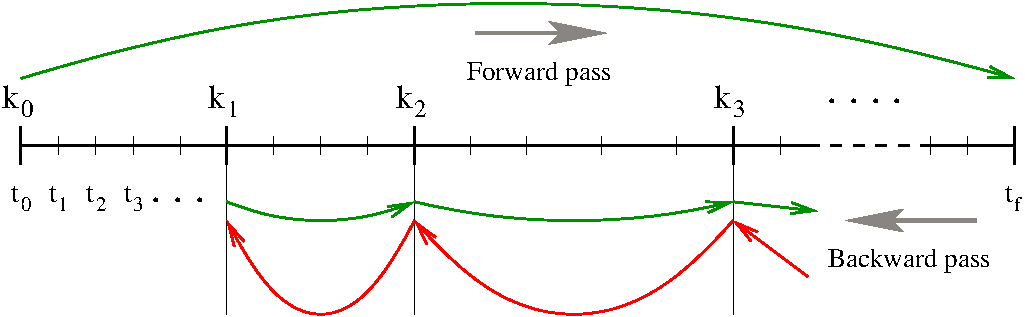
\includegraphics[width=4in]{ckpnt}}
\caption {Illustration of the checkpointing algorithm for generation of 
  the forward solution during the integration of the adjoint system.}
\label{f:ckpnt}
\end{figure}

This approach transfers the uncertainty in the number of integration
steps in the forward integration phase to uncertainty in the final
number of checkpoints.  However, $N_c$ is much smaller than the number
of steps taken during the forward integration, and there is no major
penalty for writing/reading the checkpoint data to/from a temporary
file.
%
Note that, at the end of the first forward integration stage, interpolation
data are available from the last checkpoint to the end of the interval
of integration.  If no checkpoints are necessary ($N_d$ is larger than the 
number of integration steps taken in the solution of (\ref{e:DAE_p})),
the total cost of an adjoint sensitivity computation can be as low as one forward
plus one backward integration.
%
In addition, {\idas} provides the capability of reusing a set of checkpoints
for multiple backward integrations, thus allowing for efficient computation of
gradients of several functionals (\ref{e:G}).

\bigskip

\index{adjoint sensitivity analysis!implementation in {\idas}|(}
Finally, we note that the adjoint sensitivity module in {\idas} provides the
necessary infrastructure to integrate backwards in time any DAE terminal value
problem dependent on the solution of the IVP (\ref{e:DAE_p}), including
adjoint systems (\ref{e:adj_eqns}) or (\ref{e:adj1_eqns}), as well as any other
quadrature ODEs that may be needed in evaluating the integrals in (\ref{e:dGdp}).
In particular, for DAE systems arising from semi-discretization
of time-dependent PDEs, this feature allows for integration of either the 
discretized adjoint PDE system or the adjoint of the discretized PDE.
\index{adjoint sensitivity analysis!implementation in {\idas}|)}
\index{adjoint sensitivity analysis!mathematical background|)}

%----------------------------------------
\section{Second-order sensitivity analysis}\label{ss:hess_sensi}
%----------------------------------------
\index{second-order sensitivity analysis}
In some applications (e.g., dynamically-constrained optimization) it may
be desirable to compute second-order derivative information. Considering 
the DAE problem (\ref{e:DAE_p}) and some model output
functional\footnote{For the sake of simplifity in presentation, we do not 
include explicit dependencies of $g$ on time $t$ or parameters $p$.
Moreover, we only consider the case in which the dependency of the 
original DAE (\ref{e:DAE_p}) on the parameters $p$ is through its initial conditions only.
For details on the derivation in the general case, see~\cite{OzBa:05}.}
$g(y)$, the Hessian $d^2g/dp^2$ can be obtained in a forward sensitivity
analysis setting as
\begin{equation*}
\frac{d^2 g}{d p^2} = \left(g_y \otimes I_{N_p} \right ) y_{pp} + y_p^T g_{yy} y_p \, ,
\end{equation*}
where $\otimes$ is the Kronecker product. The second-order sensitivities are
solution of the matrix DAE system:
\begin{equation*}
  \begin{split}
  & \left( F_{\dot y} \otimes I_{N_p} \right) \cdot \dot y_{pp}  +
  \left( F_y        \otimes I_{N_p} \right) \cdot y_{pp}       +
  \left( I_N \otimes {\dot y}_p^T \right) \cdot \left( F_{\dot y \dot y} \dot y_p + F_{y \dot y} y_p \right) +
  \left( I_N \otimes y_p^T        \right) \cdot \left( F_{y \dot y}      \dot y_p + F_{y y}      y_p \right) = 0 \\
  & y_{pp}(t_0) = \frac{\partial^2 y_0}{\partial p^2} \, , \quad 
  \dot y_{pp}(t_0) = \frac{\partial^2 \dot y_0}{\partial p^2} \, ,
  \end{split}
\end{equation*}
where $y_p$ denotes the first-order sensitivity matrix, the solution of $N_p$ 
systems (\ref{e:sens_eqns}), and $y_{pp}$ is a third-order tensor.
%%
It is easy to see that, except for situations in which the number of parameters
$N_p$ is very small, the computational cost of this so-called {\em forward-over-forward} 
approach is exorbitant as it requires the solution of $N_p + N_p^2$ additional
DAE systems of the same dimension as (\ref{e:DAE_p}).

A much more efficient alternative is to compute Hessian-vector products using
a so-called {\em forward-over-adjoint} approach. This method is based on using
the same ``trick'' as the one used in computing gradients of pointwise
functionals with the adjoint method, namely applying a formal directional forward 
derivation to the gradient of (\ref{e:dGdp}) (or the equivalent one for a pointwise 
functional $g(T, y(T))$). With that, the cost of computing a full Hessian is roughly 
equivalent to the cost of computing the  gradient with forward sensitivity analysis.
However, Hessian-vector products can be cheaply computed with one additional adjoint solve.

As an illustration\footnote{The derivation for the general DAE case is too
involved for the purposes of this discussion.}, consider the ODE problem  
\begin{equation*}
{\dot y}  = f(t,\,y) \, , \quad y(t_0)  = y_0(p) \, ,
\end{equation*}
depending on some parameters $p$ through the initial conditions only and
consider the model functional output $G(p) = \int_{t_0}^{t_f} g(t,y) \, dt$.
It can be shown that the product between the Hessian of $G$ (with respect to the 
parameters $p$) and some vector $u$ can be computed as
\begin{equation*}
  \frac{\partial^2 G}{\partial p^2} u = 
  \left[ \left(\lambda^T \otimes I_{N_p} \right) y_{pp}u + y_p^T \mu \right]_{t=t_0} \, ,
\end{equation*}
where $\lambda$ and $\mu$ are solutions of
\begin{equation}
  \begin{split}
    &-\dot\mu = f_y^T\mu + \left(\lambda^T \otimes I_n \right) f_{yy} s \, ; \quad \mu(t_f) = 0 \\
    &-\dot\lambda = f_y^T\lambda + g_y^T \, ; \quad \lambda(t_f) = 0 \\
    &\dot s = f_y s \, ; \quad s(t_0) = y_{0p} u .
  \end{split}
\end{equation}
In the above equation, $s = y_p u$ is a linear combination of the columns of the
sensitivity matrix $y_p$. The {\em forward-over-adjoint} 
approach hinges crucially on the fact that $s$ can be computed at the cost of 
a forward sensitivity analysis with respect to a single parameter (the last 
ODE problem above) which is possible due to the linearity of the forward
sensitivity equations (\ref{e:sens_eqns}).

Therefore (and this is also valid for the DAE case), the cost of computing the 
Hessian-vector product is roughly that of two forward and two backward integrations 
of a system of DAEs of size $N$.
For more details, including the corresponding formulas for a pointwise model
functional output, see the work by Ozyurt and Barton~\cite{OzBa:05} who discuss
this problem for ODE initial value problems. As far as we know, there is no
published equivalent work on DAE problems. However, the derivations given
in~\cite{OzBa:05} for ODE problems can be extended to DAEs with some careful
consideration given to the derivation of proper final conditions on the 
adjoint systems, following the ideas presented in~\cite{CLPS:03}.

\bigskip

\index{second-order sensitivity analysis!support in {\idas}|(}
To allow the {\em foward-over-adjoint} approach described above, {\idas} provides support for:
\begin{itemize}
\item the integration of multiple backward problems depending on the same
  underlying forward problem (\ref{e:DAE_p}), and
\item the integration of backward problems and computation of backward quadratures
  depending on both the states $y$ and forward sensitivities (for this particular 
  application, $s$) of the original problem (\ref{e:DAE_p}).
\end{itemize}
\index{second-order sensitivity analysis!support in {\idas}|)}
